\documentclass[dvipdfmx]{jsarticle}

% 警告消す用
\usepackage{silence}
\WarningFilter{caption}{Unknown document}

% 文字
\usepackage{ulem}
\usepackage{url}
\usepackage{typearea}
\usepackage{enumitem}
\usepackage{ascmac}
\usepackage{fancybox}
% 記号
\usepackage{latexsym}
\usepackage{amssymb}
% 数式
\usepackage{multirow}
\usepackage{bm}
\usepackage{amsmath}
\usepackage{mathtools}
% 画像
\usepackage[dvipdfmx]{graphicx}
\usepackage{here}
% 表
\usepackage{multicol}
% 段落
\usepackage[hang,small,bf]{caption}
\usepackage[subrefformat=parens]{subcaption}
% フォント,カラー
\usepackage[T1]{fontenc}
\usepackage[dvipdfm]{color}
\usepackage[figurename=Fig.,tablename=Tab.]{caption}
\newcommand{\eqlab}[1]{Eq.\ref{eq:#1}}%式の参照構文
\newcommand{\figlab}[1]{Fig.\ref{fig:#1}}%図の参照構文
\newcommand{\tablab}[1]{Tab.\ref{tab:#1}}%表の参照構文
\captionsetup{compatibility=false}
\catcode`_ = \active
\newcommand_[1]{\sb{\mathrm{ #1}}}

\typearea{12}

\begin{document}
\section{理論および実験の背景}
\subsection{放電の形態}
\subsubsection*{放電の電圧-電流特性}
放電は電流の大きさに応じて形態が段階的に変化する。初期の暗流やタウンゼント放電から始まり、前期グロー、正規グロー、異常グロー、最後にアーク放電へと至る。各領域では発光状態や電圧特性に明確な違いがある。\figlab{1}に一般的な電流-電圧特性を示す
 
 \begin{figure}[H]
 \centering
 \includegraphics[scale=0.4]{assets/IV-1.png}
 \caption{Current–Voltage Characteristics of Gas Discharge at Low Pressure}\label{fig:1}
 \end{figure}
図中、$I < 10^{-10}\,\mathrm{[A]}$ では暗流が流れる。暗流とは、外部電界印加下で自然放射線や熱電子によって生じたわずかなキャリアが移動することで生じる微小電流であり、発光を伴わない。電圧に対して電流は指数的に増加するが、放電はまだ開始していない。

$I \approx 10^{-10}\,\mathrm{[A]}$ 付近において、絶縁破壊が生じる。電子が十分に加速されて気体分子を電離できるようになり、放電が開始する。この時点で電子の移動が活発化するため、電流が急増し、電圧は低下する。

$I = 10^{-10} \sim 10^{-5}\,\mathrm{[A]}$ の領域ではタウンゼント放電が支配的となる。この領域では電子衝突による雪崩電離(Townsend電子雪崩)が進行するが、発光はほとんど見られない。電圧はおおよそ一定に保たれる。

$I = 10^{-5} \sim 10^{-4}\,\mathrm{[A]}$ では前期グロー放電が生じる。これはタウンゼント放電から正規グロー放電へ移行する中間的な領域であり、発光が部分的に現れる。電流増加に伴い電圧は低下する。
$I = 10^{-4} \sim 10^{-1}\,\mathrm{[A]}$ では正規グロー放電が成立する。発光が電極全体に広がり、陰極表面全域が光る。電圧はほぼ一定に維持され、安定した放電状態となる。正規グロー放電時の放電の様子を\figlab{2}に示す。

\begin{figure}[H]
 \centering
 \includegraphics[scale=0.4]{assets/glow-discharge.png}
 \caption{Potential distribution in glow discharge}\label{fig:2}
\end{figure}

正規グロー放電では、電極間に特徴的な発光領域と暗部が形成される。陰極直近にはカソードグローが現れ、その外側に負グローが続く。さらに進むとファラデー暗部があり、その先には均一な発光を示す陽光柱(positive column)が広がる。これらの領域は、電子エネルギー分布や電場強度の違いに対応しており、電流密度と電圧分布を反映している。


$I = 10^{-1} \sim 10^{0}\,\mathrm{[A]}$ では異常グロー放電に移行する。この領域では陰極表面がすでに飽和しているため、さらなる電流増加にはより大きな電圧が必要となり、電圧が再び上昇する。

最後に、$I > 10\,\mathrm{[A]}$ ではアーク放電が発生する。強い白色発光と高温プラズマを伴い、電圧は急激に低下し、大電流が流れる。アークは強い熱を発生するため、溶接などの応用に利用される。
\section{実験方法}
    \subsection{低気圧放電の特性}
        \subsubsection*{$I$-$V$特性の測定}
            放電電流を変化させた場合の印加電圧の変化を測定する。以下の通りに実験をした。
            \begin{enumerate}[label=\textbf{(\arabic*)}]
            \item \figlab{3a}に示す実験装置を準備する。
            \item 電極距離が5[cm]となるように調整する。
            \item 吸引を開始し、管内気圧が100[Pa]となるように、ピラニーゲージを参照しながらリークバルブを調整する。
            \item 電圧を印加し、ポンプの油を温めることと、管内の空気を電離させることを目的として5分ほど放電させる。
            \item 電圧を変化させて電流を変化させ、電流計と電圧計の値を読む。
            \end{enumerate}
        \subsubsection*{$V_s - p$特性の測定}
            \begin{enumerate}[label=\textbf{(\arabic*)}]
            \item \figlab{3a}に示す実験装置を準備する。
            \item 電極距離を3,5,7[cm]になるようにピラニーゲージを参照しながらリークバルブを調整する。
            \item 吸引を開始し、管内気圧が20[Pa]となるように、ピラニーゲージを参照しながらリークバルブを調整する。
            \item 電圧を印加して、放電開始電圧$V_s$を読む。
            \item 管内気圧が2700[Pa]になるまで繰り返す。
            \end{enumerate}      
        \subsubsection*{実験装置}
            本実験で用いた実験装置を\tablab{e1}に示す。

        
    \subsection{プラズマの測定と放電管内のプラズマの特性}
        \subsubsection*{$V_p - I_p$特性の測定}
            \begin{enumerate}[label=\textbf{(\arabic*)}]
            \item \figlab{3b}に示す実験装置を準備する。
            \item 放電管内をArガスで満たし、圧力を測定する。
            \item 直流電源電圧を変化させ、電流を測定し、$V_p - I_p$特性を測定する。
            \item 計測した$V_p - I_p$特性から、電子密度$n_e$と電子温度$T_e$を求める。
            \end{enumerate}
        \subsubsection*{実験装置}
            本実験で用いた実験装置を\tablab{e2}に示す。

    \begin{figure}[H]
    \begin{minipage}[b]{0.45\linewidth}
    \centering
    \includegraphics[keepaspectratio, scale=0.7]{assets/e1.png}
    \subcaption{Low-Pressure Gas Discharge Circuit}\label{fig:3a}
    \end{minipage}
    \begin{minipage}[b]{0.45\linewidth}
    \centering
    \includegraphics[keepaspectratio, scale=0.7]{assets/e2.png}
    \subcaption{Plasma Generator and Measurement Circuit}\label{fig:3b}
    \end{minipage}
    \caption{experimental measurement circuit}
    \end{figure}
  
\section{実験結果}
    \subsection{低気圧放電の特性}
        \subsubsection*{$I$-$V$特性の測定}
            本実験では、管内気圧100[Pa]、電極間距離5[cm]に設定し、実験を行った。
            測定結果を\tablab{1}に示す。
            
            \begin{table}[H]
                \centering
                \caption{Measured $I$–$V$ characteristics of the discharge tube at 100 Pa}\label{tab:1}
                    \begin{tabular}{cc|cc}
                    \hline
                    Discharge current & Applied voltage & Discharge current & Applied voltage \\
                    $I$ [mA]          & $V$ [V]         & $I$ [mA]          & $V$ [V] \\
                    \hline
                    0.10 & 675 & 1.80 & 505 \\
                    0.35 & 462 & 2.00 & 385 \\
                    0.40 & 420 & 2.10 & 385 \\
                    0.49 & 483 & 2.21 & 383 \\
                    0.60 & 480 & 0.30 & 382 \\
                    0.72 & 489 & 2.40 & 381 \\
                    0.80 & 490 & 2.50 & 380 \\
                    0.91 & 495 & 2.61 & 381 \\
                    1.02 & 500 & 2.75 & 381 \\
                    1.12 & 509 & 2.90 & 381 \\
                    1.20 & 519 & 3.05 & 380 \\
                    1.30 & 525 & 3.12 & 380 \\
                    1.50 & 499 & 3.20 & 380 \\
                    1.60 & 499 & 3.40 & 380 \\
                    1.70 & 500 & 3.60 & 380 \\
                    \hline
                    \end{tabular}%
            \end{table}

            
            \begin{figure}[H]
            \centering
            \includegraphics[scale=0.7]{assets/e2-2.bmp}
            \caption{Measured $I$–$V$ characteristics of the discharge tube at 100 Pa}\label{fig:4}
            \end{figure}
            
            
        \subsubsection*{$V_s - p$特性の測定}
            
            \begin{table}[H]
            \centering
            \caption{Breakdown voltage as a function of pressure $p$ and electrode distance $d$}
            \label{tab:2}
            \begin{tabular}{cccc}
            \hline
                                & \multicolumn{3}{c}{Electrode distance $d$ [cm]} \\ \hline
            Gas Pressure $p$ [Pa] & 3              & 5              & 7             \\ \hline
            20                    & 390            & 360            & 430           \\
            40                    & 380            & 430            & 500           \\
            60                    & 430            & 500            & 580           \\
            80                    & 460            & 570            & 640           \\
            100                   & 500            & 620            & 730           \\
            200                   & 650            & 850            & 1100          \\
            400                   & 960            & 1250           & 1550          \\
            600                   & 1400           & 1800           & 2100          \\
            800                   & 1650           & 2300           & 2550          \\
            1000                  & 1850           & 2600           & 3100          \\
            2000                  & 3200           & 4100           & 4650          \\
            2700                  & 3850           & 4900           & 5150          \\ \hline
            \end{tabular}
            \end{table}

           
    \subsection{プラズマの測定と放電管内のプラズマの特性}
        測定結果を\tablab{3}に示す。また、$V_p - I_p$特性図を\figlab{6}に示す。

        \begin{table}[H]
        \centering
        \caption{Measured $V_p - I_p$ characteristics of the discharge tube}
        \label{tab:3}
        \resizebox{\columnwidth}{!}{%
        \begin{tabular}{ccc|ccc}
        \hline
        \begin{tabular}[c]{@{}c@{}}Probe Voltage\\ $V_p$[V]\end{tabular} &
        \begin{tabular}[c]{@{}c@{}}Shunt Voltage\\ $V_{Ip}$[V]\end{tabular} &
        \begin{tabular}[c]{@{}c@{}}Probe Current\\ $I_p$[mA]\end{tabular} &
        \begin{tabular}[c]{@{}c@{}}Probe Voltage\\ $V_p$[V]\end{tabular} &
        \begin{tabular}[c]{@{}c@{}}Shunt Voltage\\ $V_{Ip}$[V]\end{tabular} &
        \begin{tabular}[c]{@{}c@{}}Probe Current\\ $I_p$[mA]\end{tabular} \\ \hline
        -147.3 & -0.212  & -0.021  & -1.188               & 59.4                 & 5.9                  \\
        -125.3 & -0.192  & -0.019  & 4.800                & 65.5                 & 6.6                  \\
        -100.9 & -0.158  & -0.016  & 10.35                & 67.3                 & 6.7                  \\
        -74.80 & -0.109  & -0.011  & 15.14                & 68.3                 & 6.8                  \\
        -49.70 & -0.0285 & -0.0029 & 20.20                & 68.2                 & 6.8                  \\
        -40.40 & 0.156   & 0.016   & 25.20                & 68.9                 & 6.9                  \\
        -35.10 & 0.437   & 0.044   & 50.20                & 69.8                 & 7.0                  \\
        -29.50 & 0.900   & 0.090   & 75.00                & 69.9                 & 7.0                  \\
        -25.10 & 1.706   & 0.17    & 100.3                & 70.0                 & 7.0                  \\
        -19.40 & 2.97    & 0.30    & 124.9                & 70.2                 & 7.0                  \\
        -15.06 & 5.09    & 0.51    & 150.0                & 70.3                 & 7.0                  \\
        -9.780 & 8.87    & 0.89    & 175.1                & 70.4                 & 7.0                  \\
        -7.940 & 24.7    & 2.5     & 200.0                & 70.5                 & 7.1                  \\
        -6.910 & 37.1    & 3.7     & 225.0                & 70.6                 & 7.1                  \\
        -5.010 & 44.3    & 4.4     & 250.0                & 70.8                 & 7.1                  \\
        -2.080 & 55.7    & 5.6     & \multicolumn{1}{l}{} & \multicolumn{1}{l}{} & \multicolumn{1}{l}{} \\ \hline
        \end{tabular}%
        }
        \end{table}

        
        \begin{figure}[H]
        \centering
        \includegraphics[scale=0.7]{assets/e1re.bmp}
        \caption{Measured $V_p - I_p$ characteristics of the discharge tube}\label{fig:6}
        \end{figure}
        
        
\section{考察}
\section{まとめ}



% \bibliographystyle{junsrt}
% \bibliography{main} 
\end{document}